\section{Fase 2: Línea base}

De la versión S en adelante, DuckDB es entre 4 y 11 veces más rápido que Pandas y entre 17 y 30 veces más rápido que SQLite sobre el mismo CSV. El orden se mantiene en las tres máquinas y en todas las versiones.

\subsection{Tiempo total por herramienta y versión}

Suma de las tres preguntas, en segundos. Cada celda es carga $+$ query acumulado. El desglose por pregunta de cada equipo está en los archivos \texttt{benchmarks\_*.csv} del repositorio.

\begin{table}[htbp]
\centering
\small
\caption{Tiempo total (carga + query) por versión, equipo y herramienta}
\label{tab:fase2-tiempos}
\begin{tabular}{llrrr}
\toprule
Versión & Equipo & Pandas & DuckDB & SQLite \\
\midrule
XS & Pc\_Martha & 1.9   & 0.7   & 5.8 \\
S  & Pc\_Martha & 29.5  & 4.0   & 97.2 \\
M  & Pc\_Jesus  & 34.5  & 5.0   & 108.2 \\
M  & Pc\_Martha & 50.0  & 6.7   & 164.6 \\
M  & Pc\_Nahin  & 143.1 & 15.3  & 445.0 \\
L  & Pc\_Jesus  & 79.1  & 11.5  & 232.8 \\
L  & Pc\_Martha & 106.5 & 15.3  & 404.0 \\
L  & Pc\_Nahin  & 288.1 & 25.9  & 776.9 \\
XL & Pc\_Jesus  & 195.4 & 27.3  & 472.6 \\
XL & Pc\_Martha & falló & falló & falló \\
XL & Pc\_Nahin  & 501.4 & 122.3 & excedió \\
\bottomrule
\end{tabular}
\end{table}

\subsection{Por qué ese orden}

\textbf{DuckDB} almacena por columnas y ejecuta de forma vectorizada y multi-hilo. Para un \texttt{GROUP BY} lee únicamente las dos o tres columnas que necesita; el resto del ancho de fila nunca toca el disco ni la RAM.

\textbf{Pandas} también es columnar en memoria y vectorizado sobre NumPy, pero es mono-hilo y paga materializar las nueve columnas, incluidas las dos de texto con los nombres de estación, que son las más caras de parsear y las que más memoria ocupan.

\textbf{SQLite} está orientado a filas. Un \texttt{GROUP BY} recorre cada registro completo y parsea los timestamps con \texttt{strftime} fila por fila. Es el comportamiento esperado: SQLite está optimizado para OLTP, es decir, buscar e insertar pocas filas por clave, no para agregar decenas de millones.

\subsection{Dónde se va el tiempo}

El desglose entre carga y consulta es la observación que justifica toda la Fase 3. En la versión XL sobre Pc\_Jesus:

\begin{table}[htbp]
\centering
\caption{Desglose carga vs. query, versión XL, Pc\_Jesus}
\label{tab:fase2-desglose}
\begin{tabular}{llrrr}
\toprule
Herramienta & Pregunta & Carga (s) & Query (s) & \% en carga \\
\midrule
Pandas & Q1 & 56.7 & 2.7  & 95\% \\
Pandas & Q3 & 57.2 & 21.6 & 73\% \\
DuckDB & Q1 & 9.0  & 0.3  & 97\% \\
DuckDB & Q3 & 8.1  & 1.4  & 85\% \\
SQLite & Q1 & 99.8 & 28.6 & 78\% \\
SQLite & Q2 & 108.8& 82.6 & 57\% \\
\bottomrule
\end{tabular}
\end{table}

La carga domina en todos los casos. Y como el protocolo obliga a recargar el archivo en cada pregunta, ese costo se paga tres veces. \textbf{El formato de almacenamiento es, entonces, la palanca de optimización más rentable disponible.}

\begin{figure}[htbp]
  \centering
  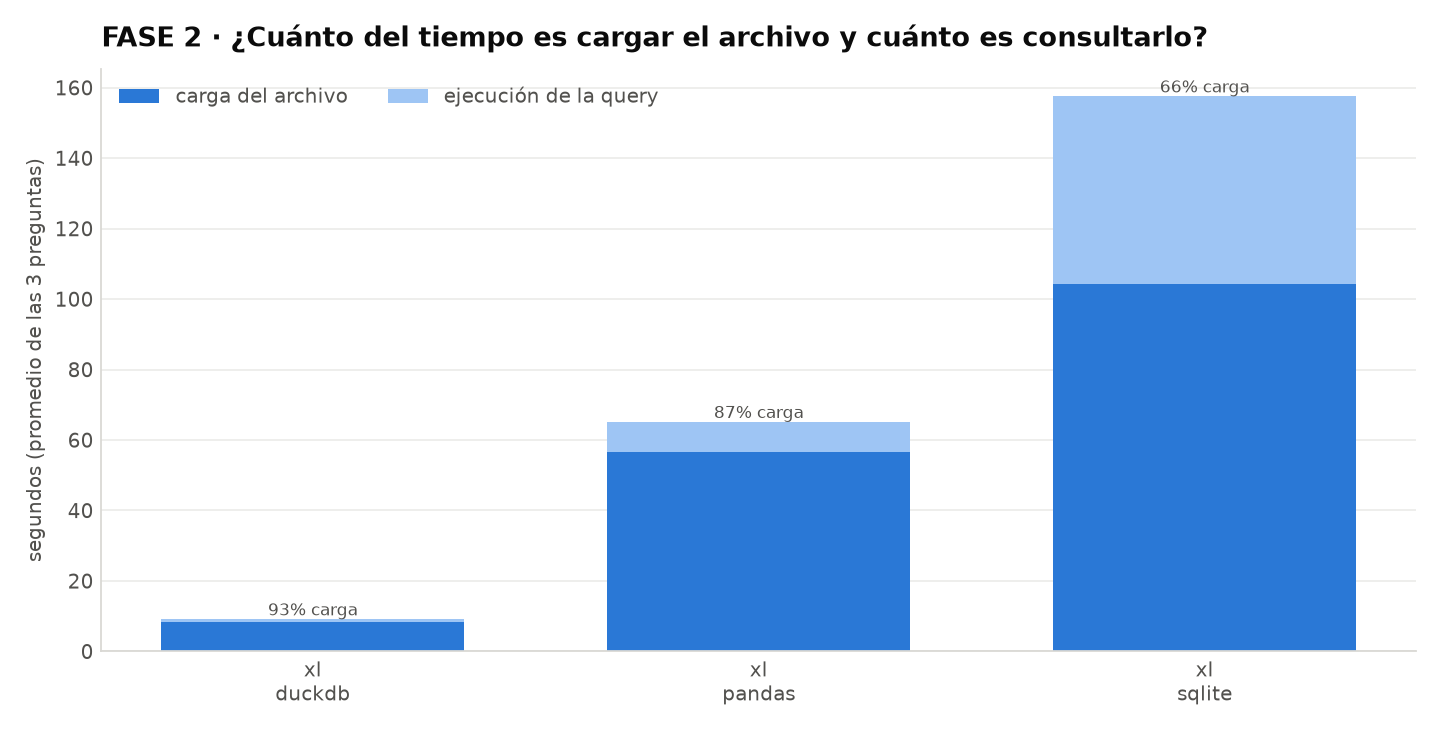
\includegraphics[width=0.75\textwidth]{figuras/fase2_carga_vs_query_pc_jesus.png}
  \caption{Reparto entre tiempo de carga y tiempo de consulta, Pc\_Jesus.}
  \label{fig:fase2-carga-query}
\end{figure}

\begin{figure}[htbp]
  \centering
  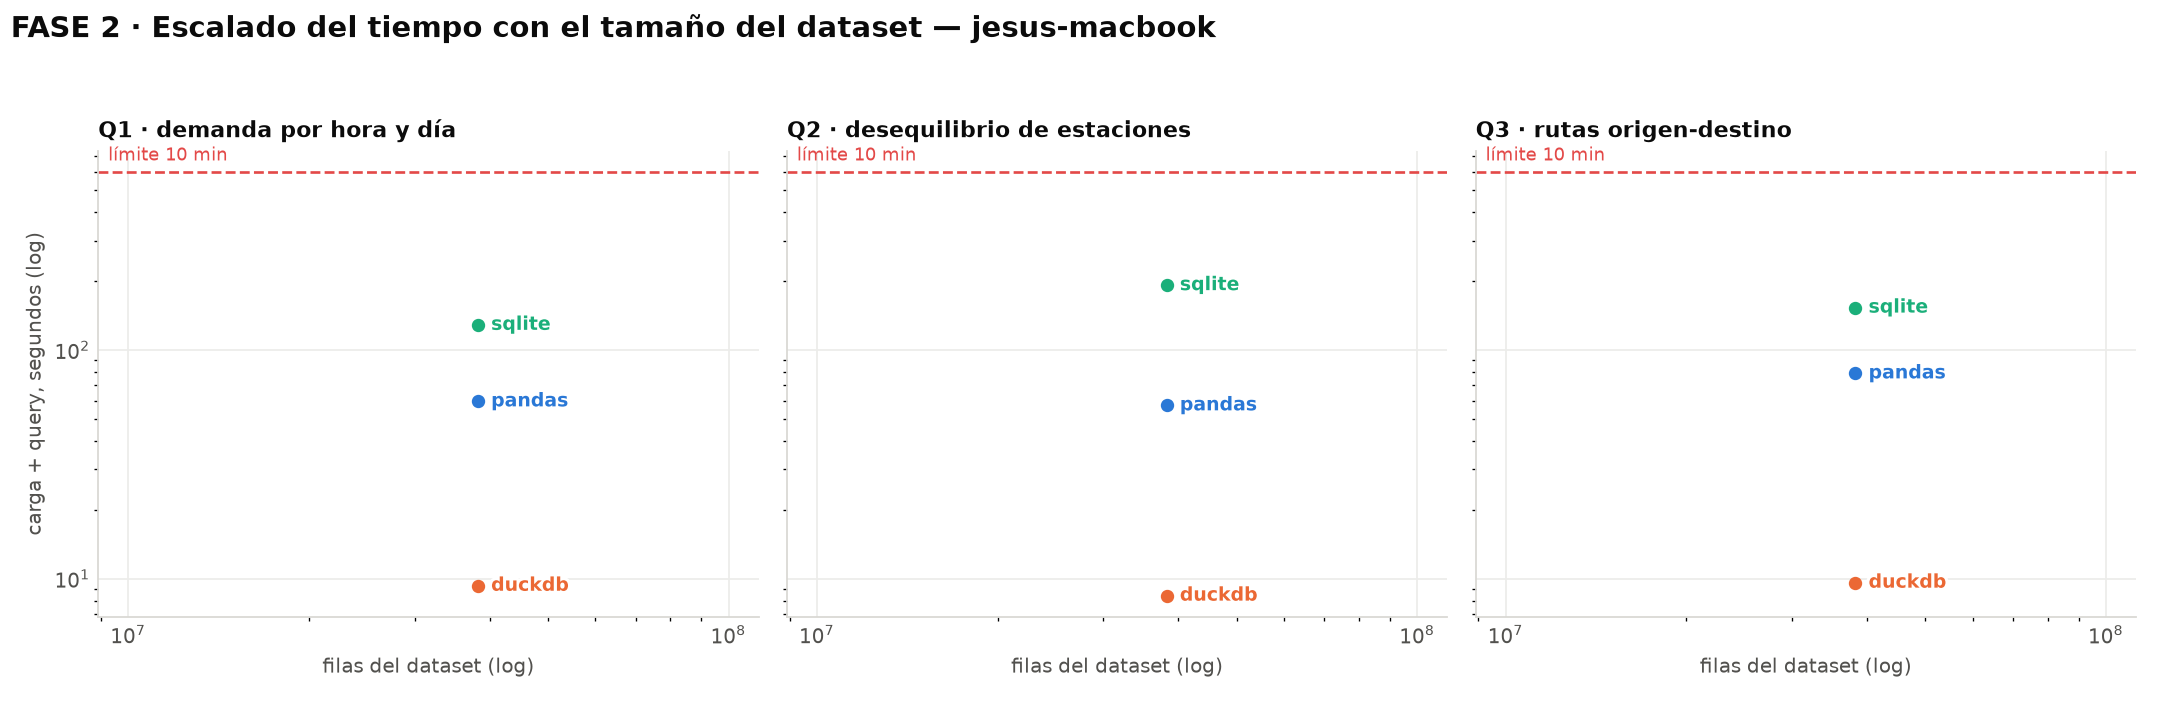
\includegraphics[width=0.75\textwidth]{figuras/fase2_escalado_pc_jesus.png}
  \caption{Escalado log-log del tiempo total contra el número de filas, Pc\_Jesus.}
  \label{fig:fase2-escalado}
\end{figure}
